% !TeX root = main.tex

\section{Songfics: o encontro das artes}\label{sec-songfics}

Consoante a \textcite{bakhtin2011}, os enunciados são únicos, irrepetíveis e
caracterizados pela heterogeneidade, o que leva à diversidade de gêneros
discursivos transformados ao longo do tempo, moldados pela interação
discursiva e variando em diferentes contextos e propósitos
comunicativos. Essas mudanças nas práticas discursivas levam à
transformação dos gêneros, resultando em atualizações em sua composição
e na maneira como são empregados. No tocante às \emph{songfics},
precisamos detalhar o conceito de reelaboração de gênero. \textcite{araujo2009},
fundamentado nas ideias de \textcite{bakhtin_os_1997}, argumenta que a
interação humana é uma das necessidades mais inerentes, resultando na
criação de diversos gêneros em vários campos discursivos aos quais
pertencemos ou com as quais interagimos, como o jurídico, jornalístico,
religioso, acadêmico, entre outros. Conforme esses contextos tornam-se
mais complexos, os próprios gêneros também se tornam mais sofisticados.

Bakhtin utilizou o termo \emph{transmutação} para descrever a
transformação de gêneros complexos, que são empregados em contextos mais
formais, como discursos, artigos e livros, a partir de gêneros
primários, usados em situações cotidianas, como conversas e cartas.
Nesse processo, quando um gênero primário se modifica para se adequar a
um contexto mais formal, muitas vezes, ele assume uma nova natureza,
desvinculando-se da realidade imediata. A transmutação (doravante
\emph{reelaboração}) é um processo constante, o qual os gêneros
complexos estão em constante evolução e adaptação para atender às
necessidades daqueles que os utilizam. No entanto, Bakhtin utilizou esse
conceito especificamente para descrever o fenômeno da formação de
gêneros complexos, que têm origem nos primários. Todavia, hodiernamente,
há casos em que gêneros secundários (complexos) também passam por
transmutação, ou seja, são reelaborados por outros gêneros secundários.

\textcite{araujo2009} ilustra o exemplo do \emph{chat}, que, além de abranger as
conversas cotidianas, também abarcam outros gêneros secundários, como a
aula, a entrevista, a enquete e o material didático, resultando na
formação de uma constelação de gêneros com objetivos variados. Isso se
diferencia das \emph{songfics}, cujo propósito geralmente é mais
específico, qual seja: (re)criar obras artístico-midiáticas, ao passo
que o \emph{chat} pode servir a uma infinidade de funções outras. Neste
caso, há uma negociação do sentido, posto que a canção, ao ser
reelaborada, perde o contato com o seu meio de circulação primário,
tornando-se parte de um novo gênero. Em outras palavras, os gêneros
discursivos têm uma memória, o que significa que eles têm raízes em
gêneros previamente estabelecidos e estão intrinsecamente ligados a um
contexto e a uma comunidade discursiva. No caso das \emph{songfics},
isso está vinculado ao \emph{fandom}.

Nessa perspectiva, a renovação dos gêneros pode assumir, em geral, duas
formas: \emph{transmutação criadora}, quando um gênero inédito, isto é,
com novo propósito comunicativo, surge a partir de outro(s); e
\emph{transmutação inovadora}, quando todo e qualquer gênero, mesmo os
mais estandardizados, comportam transformações, sem que essas o
transformem em um novo gênero. Em essência, as \emph{songfics} (também
conhecidas como \emph{canções-fic}, \emph{ficsongs} ou \emph{fic
músicas}) são narrativas de ficção que incorporam letras de canções, as
quais podem ser intercaladas entre as seções da história ou integradas
ao próprio enredo. A narrativa pode até mostrar personagens ouvindo a
música no rádio e reagindo de acordo ou apresentar momentos da história
nos quais a música desempenha um papel relevante. Além disso, as
\emph{songfics} podem incluir recursos multimodais, como
\emph{hiperlinks}, GIFs, imagens e vídeos, juntamente às estratégias
intertextuais discutidas anteriormente.

Em relação às \emph{fanfictions}, a principal diferença não está no
suporte, mas na maneira como as \emph{songfics} incorporam e utilizam
letras de músicas como parte integrante da narrativa. A diversidade de
abordagens e manipulações nas histórias é vasta e depende dos interesses
e desejos dos \emph{fandoms} que estão espalhados pela internet. Cada um
deles desenvolve suas próprias interpretações criativas e variações das
narrativas, criando uma rede rica e multifacetada de conteúdo dentro
desse universo, de modo que cada sujeito apresenta seu assento
valorativo diante do tema a partir de sua própria dimensão ideológica.
Nessa direção, \textcite{jenkins_textual_1992} aponta dez maneiras pelas quais esse
processo é realizado:

\begin{enumerate}
\def\labelenumi{\arabic{enumi})}
\item
  Recontextualização, que consiste no preenchimento de lacunas na
  história original, explorando as ações não descritas ou mesmo a
  psicologia das personagens;
\item
  Expansão da Linha Temporal, que se refere à narração de eventos não
  mencionados no passado ou futuro da narrativa, sem contradizer o
  cânone;
\item
  Refocalização, que narra a história a partir da perspectiva de
  personagens secundárias ou marginalizadas;
\item
  Realinhamento Moral, a qual compreende transformar vilões em
  protagonistas e explorar suas perspectivas, razões etc.;
\item
  Troca de Gênero, que enfatiza elementos como o romance em histórias
  que não o destacam;
\item
  Crossovers, a prática de unir personagens e cenários de diferentes
  histórias;
\item
  Deslocamento de Personagem, quando personagens são retirados de seus
  contextos originais e então inseridos em situações diferentes;
\item
  Personalização, que se refere à transposição de personagens para novos
  ambientes, a ponto de se trocar características físicas, nome, idade
  etc.;
\item
  Intensificação Emocional, de modo que momentos de crise emocional são
  focalizados nas fics, como um término ou situação traumática, por
  exemplo;
\item
  Erotização, ao serem explorados aspectos eróticos da narrativa, sem
  restrições editoriais e, neste caso, restrito ao público maior de
  idade.
\end{enumerate}

Independentemente das diferentes formas de criação literária, o conceito
de dialogismo de \textcite{bakhtin2011} está sempre presente. Esse fenômeno
reflete a natureza inerente da interação que rege nossos contatos
sociais, sendo fundamental para a capacidade de formular e expressar
qualquer discurso ou enunciado. É o diálogo constante entre vozes,
pontos de vista e influências que enriquece e molda a complexidade das
criações literárias, como as \emph{fics}, e, de fato, todas as formas de
comunicação humana. No diagrama abaixo, apresentamos um breve fluxo que
descreve a formação das \emph{songfics}:

\begin{figure}[htbp]
    \centering
    \begin{minipage}{.75\textwidth}
    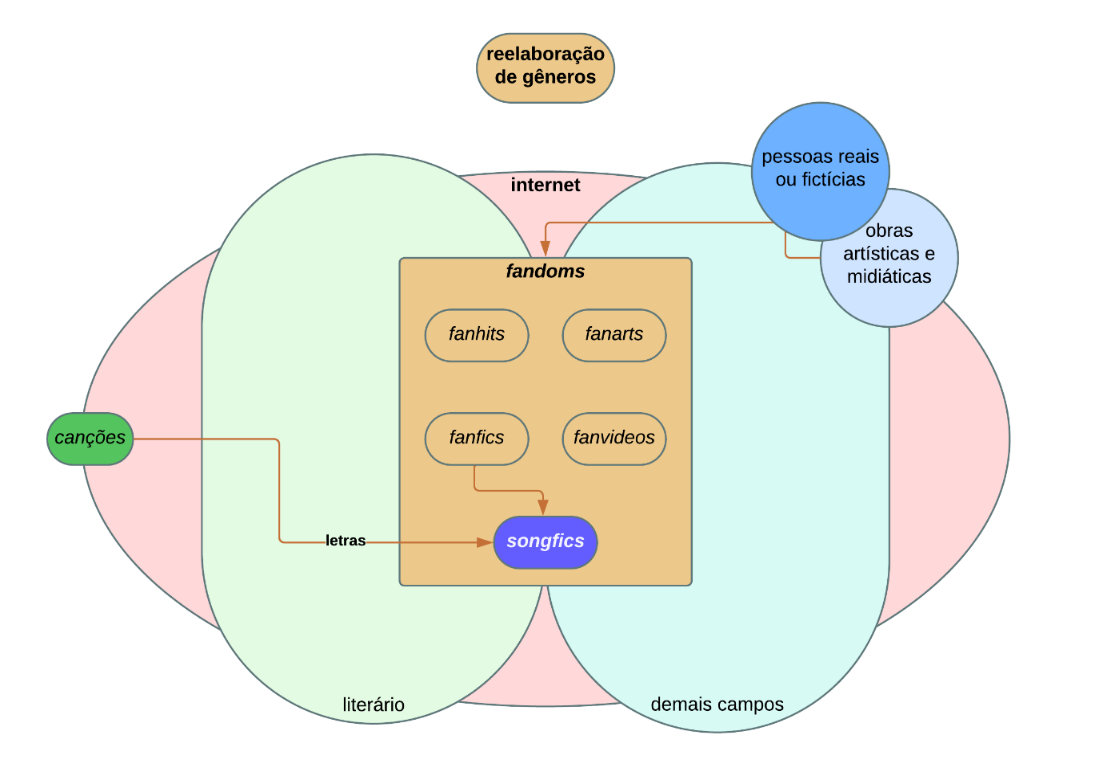
\includegraphics[width=\textwidth]{fig01.png}
    \caption{O surgimento das songfics.}
    \label{fig-01}
    \source{Elaboração própria.}
    \end{minipage}
\end{figure}

É importante notar que o ambiente predominante em que essas criações
circulam é a internet (em rosa), que serve como o local de encontro e de
interação para diversos \emph{fandoms} (comunidades de fãs) existentes.
Esses grupos de fãs produzem uma variedade de conteúdos com base em
pessoas reais ou fictícias (em azul) e em obras artísticas e midiáticas
(azul-claro), que constituem o principal \emph{input} para a criação de
\emph{fanhits}, \emph{fanarts}, \emph{fanvideos}, \emph{fanfics} e
outros tipos de produções. Estas últimas, além de serem influenciadas
por esses elementos, também são alimentadas pelas letras de canções (em
verde), que servem de inspiração para a criação das \emph{songfics} (em
roxo), por meio de um processo de \emph{reelaboração}. Esse diagrama
ilustra como as \emph{songfics} se encaixam em um contexto mais amplo de
criação de conteúdo dentro dos \emph{fandoms}, destacando a interconexão
entre diferentes formas de expressão criativa. De modo mais específico,
vejamos, na \Cref{fig-02}, o fluxo desse gênero:


\begin{figure}[htbp]
    \centering
    \begin{minipage}{.5\textwidth}
    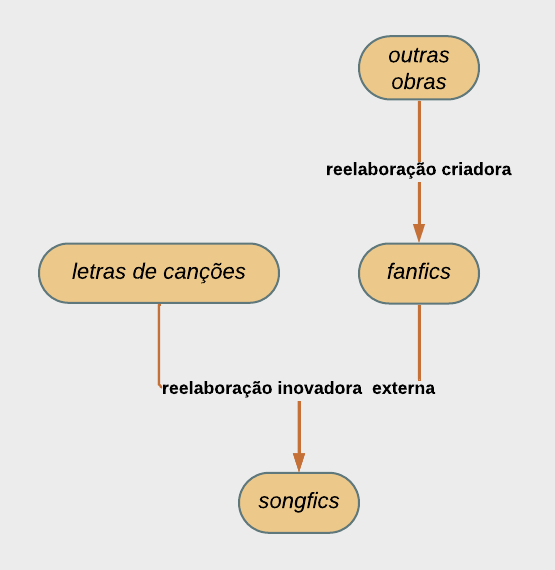
\includegraphics[width=\textwidth]{fig02.png}
    \caption{Reelaboração.}
    \label{fig-02}
    \source{Elaborado com base em \textcite{araujo2009}.}
    \end{minipage}
\end{figure}

De forma ampla, as \emph{fanfictions} são escritas com base em obras
pré-existentes, como filmes, séries, jogos etc., com o objetivo de
expandir, recriar ou modificar o universo ficcional originário,
resultando na criação de uma literatura não oficial. Esse processo pode
ser considerado como uma forma de \emph{reelaboração criativa}, uma vez
que um gênero é gerado a partir de outro. Nesse contexto, o propósito e
a função são alterados, já que as \emph{fanfics} lançam uma nova
perspectiva sobre a obra e atendem a um público específico, os
\emph{fandoms}, que empregam diversas estratégias de reinterpretação
para personalizar suas criações. Nessa cultura participativa, como
descrita por \textcite{jenkins2009}, os consumidores (\emph{ficwriters}, no caso
das \emph{fanfics}) interagem ativamente com os produtores das obras
originais, seguindo um novo conjunto de regras e níveis de poder. Os
meios de comunicação contemporâneos democratizaram esse processo. No
entanto, no contexto das \emph{songfics}, os fanfiqueiros decidem
incorporar outro elemento às suas histórias: as letras de canções. Isso
leva à \emph{reelaboração inovadora externa}, uma vez que um gênero
(\emph{fanfiction}) passa a incluir elementos de outro gênero (letras de
músicas). Isso ocorre sem comprometer a função original das
\emph{fanfics}, que é recriar outras obras artísticas. O que acontece,
na verdade, é a introdução de um novo elemento capaz de transformar
internamente um gênero já flexível por natureza.

Com recursos intergenéricos, intertextuais e multimodais, os
\emph{ficwriters} têm à disposição uma nova forma de expressão
artística: a \emph{songfic}. Este gênero permite que três vozes ressoem:
a voz da referência primária (a obra original, a pessoa etc.), a voz da
canção e, não menos importante, a voz do próprio autor que a escreve. O
diálogo entre essas forças coloca a \emph{songfic} em constante fluxo
dialógico da língua, enriquecendo a diversidade das criações literárias.
Com o público infanto-juvenil, portanto, constrói-se um leque de
possibilidades deveras abrangente, em um campo ainda preterido pela
academia e críticos mais tradicionais. Na vida escolar, a incorporação
de recursos e tecnologias multimidiáticas tem ocorrido gradualmente,
porém em um ritmo menos acelerado em comparação ao cotidiano fora das
instituições de ensino, de acordo com \textcite{damiani2016}. Com isso em mente,
a seguir, vejamos a análise de um exemplar de \emph{songfic} que dialoga
com múltiplas linguagens e mídias.